\newpage
\subsection{Agile Project Management \& Lean UX} \label{Agile Project Management & Lean UX}
% Explain what Agile is, why it is good, how it is adopted and why it is the new standard =>
% statistics. Mention that agile with a focus on design is not that easy and that there are mulitple
% popular ways. 
As traditional project management has its limitations, Agile and Lean UX provide effective
methodologies that can help to optimize the workflow.

\subsubsection{Agile Manifesto}

What being Agile means is defined in the Agile Manifesto. Created in 2001, it is a set of values and
principles, written by 17 software developers, that aim to improve the way software is made. The
four core values are:
\begin{enumerate}
    \item Individuals and interactions over processes and tools
    \item Working software over comprehensive documentation
    \item Customer collaboration over contract negotiation
    \item Responding to change over following a plan
\end{enumerate}
\directcite{beckManifestoAgileSoftware2001}

So, only by looking at these values, it immediately becomes clear how different this approach is.
Instead of having separate teams, Agile promotes collaboration between all members. Instead of a
fixed scope and plan, Agile is about being able to react to change and feedback.

\subsubsection{Agile Frameworks}
To implement Agile, there are different frameworks that can be used. These include Kanban, Lean or
Scrum, while the latter is the most popular for software development. Scrum tries to realize the Agile
vision by breaking down the project into smaller, manageable parts called sprints. Each sprint is
about 2-4 weeks long and aims to \textit{increment} the product a little bit in each iteration
\vglcite[7]{schwaberScrumGuideDefinitive2020}

The basic idea is that after each sprint, the team has a working version of the product that can be
tested and improved the next sprint. Of course in the beginning the product is basic, but it
iteratively grows more mature.

In contrast to the Waterfall model, where the scope is fixed, Agile has a fixed time and budget.
This illustration shows the difference between the two models:
\begin{figure}[H]
    \centering
    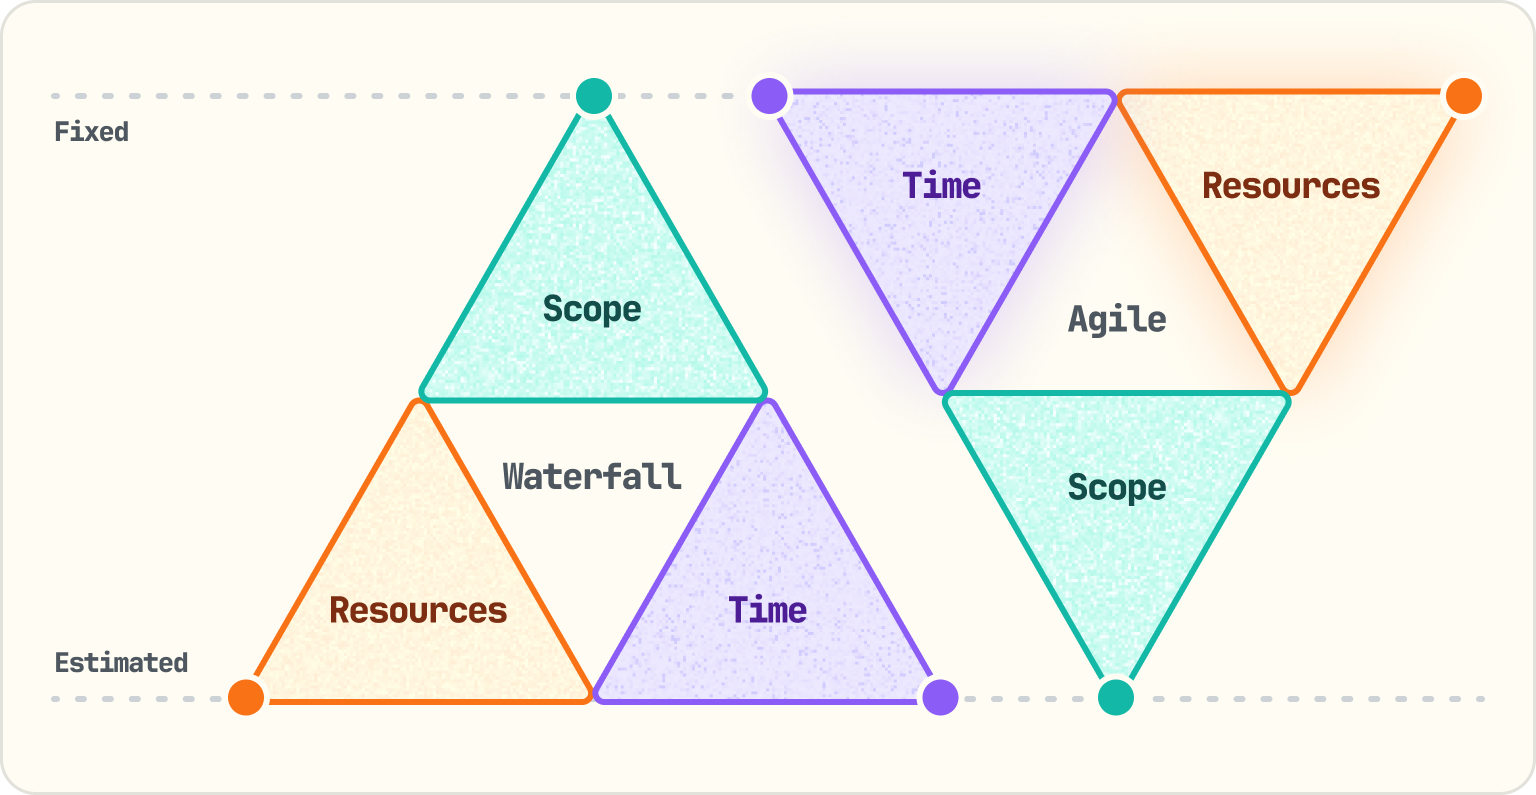
\includegraphics[width=300pt]{Chapter 3/Agile Triangle.png}
    \caption{Project management triangle (Source: own illustration based on Atlassian https://www.atlassian.com/agile/agile-at-scale/agile-iron-triangle)}
\end{figure}
% NOTE DONE:  Mention the triangle:
% https://www.ecosia.org/images?addon=firefox&addonversion=5.1.1&q=agile+vs+traditional+triangle#id=88D37B800865C1E5C05FA187E99967170A4BCFEF 

Scrum also relies on meaningful meetings, like the daily stand-up, where the whole developer team
comes together discussing what the individual members did the previous day, what they are going to
do today and whether there are any blockers. This way, everyone is involved and can help where help
is needed. \vglcite[9]{schwaberScrumGuideDefinitive2020}

\begin{figure}[H]
    \centering
    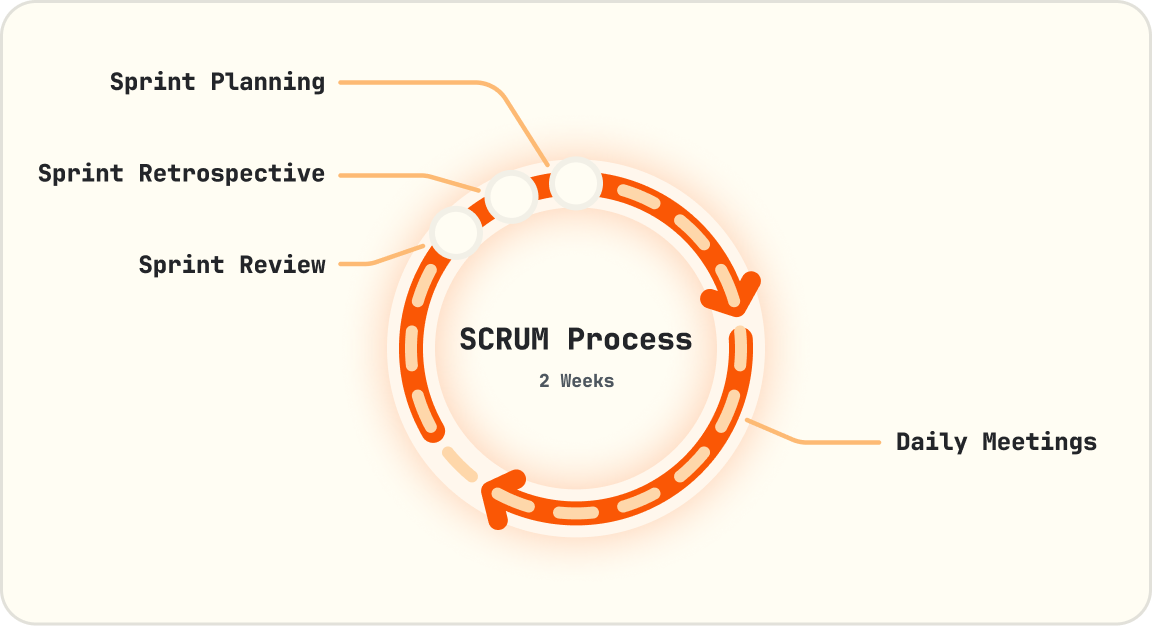
\includegraphics[width=300pt]{Chapter 3/Scrum Process.png}
    \caption{Scrum process (Source: own illustration based on Atlassian https://www.atlassian.com/de/agile/scrum/sprints)}
\end{figure}
% NOTE DONE: Add graphics of scrum process

That brings the design of web projects a lot closer to the desired outcome. Iteratively building the
solution allows for continuous adaptation to feedback and change. Moreover, it ensures a fitting and
working product at all times. However, where does design fit in all of this? This is where Lean UX
comes in. 

\subsubsection{Lean UX}
% For example Dual Track Agile. Then explain why Lean UX has the best things for my
% ways since small teams work well with it to be integrated, so also design can be as iterative as
% development. Especially working well in small teams. Maybe mention Dual-Track Agile and also the
% risk of it creating silos again.

% Hmm lets skip dual track agile and not mention that much about it. It is however also mentioned in
% Lean UX so lets see how I can integrate that.
In their book \textit{Lean UX}, Jeff Gothelf and Josh Seiden describe how Lean UX is a way of
integrating UX/UI design into Agile software projects. They build on the core values of the Agile
Manifesto and prove that design can be as iterative as development.

The main idea is to work in small, cross-functional teams that build a shared understanding of the
product, the customers and the business goals. These multidisciplinary teams work closely together
minimizing the need for long handoffs. Also, through diverse perspectives, the potential to create
better solutions is maximized. 
\vglcite[24, 26]{gothelfLeanUXProduktentwicklung2016}

So, how does this process actually look like? The process is broken down into four main parts:

% NOTE: Maybe add a graphic of the Lean UX process

\textbf{Outcomes, Assumptions, Hypotheses} \\ % (Lean UX page 38)
Designers and non-designers get together to formulate assumptions, guided by high quality problem
statements. These assumptions contain statements about what the team believes might be true for the
product given the constraints of the problem statement. Then, assumptions are turned into hypotheses
that can be designed and tested by their expected outcomes. After prioritizing the hypotheses by
looking at their value and risk, the team can start designing.
\vglcite[38, 62]{gothelfLeanUXProduktentwicklung2016}

\textbf{Design it} \\
Designers call informal collaborative design meetings or so-called Design Studios, where the whole
team does brainstorming and sketching. Another idea mentioned are one-to-one, designer-developer sessions.
In these meetings everyone gets to come up with ideas and sketches of low-fidelity. That way the
designers have a great pool of diverse ideas to work with.
\vglcite[63,67]{gothelfLeanUXProduktentwicklung2016} 

\textbf{Create an MVP} \\
Creating an Minimal Viable Product (MVP) has the goal of learning as much about the target audience
as possible in the least amount of time. With the hypotheses and the designs in hand an MVP can be
created by asking a question like \textit{What is the least amount of work we can do to achieve
    this?}. By doing this, no resources are wasted to do something which brings no or little value and
the team can implement features quickly and informed.
\vglcite[92, 93]{gothelfLeanUXProduktentwicklung2016}

\textbf{Research \& Learning} \\
With the MVP in place, testing can begin to validate assumptions and hypotheses. With collaborative
research techniques or customer feedback, again every team member gets in contact with this aspect
of building a product, adding to the shared understanding of it. These learnings feed the next cycle
of this process. \vglcite[110, 113]{gothelfLeanUXProduktentwicklung2016} \\

It can be seen that this process includes several fun and innovative methods that push collaboration
even further. The Design Studio for instance, brings the whole team together to sketch out ideas for
specific problems. Although these sessions are led by a designer, everyone contributes and is part
of the design process. \vglcite[68,69]{gothelfLeanUXProduktentwicklung2016}

Another proposed method is called collaborative design, where a minimum of two members come together
to work on a specific problem and sketch ideas rather informally. Often these informal discussions
result in the best and most creative solutions.
\vglcite[66]{gothelfLeanUXProduktentwicklung2016}

These practices all lead to more shared knowledge and understanding and help developers be part of
the design process and vice versa. The whole team moves from blindly implementing features to seeing
the holistic picture and focusing on solving real-world problems - the team culture is positively
different.

As suggested by the authors, this process can also be integrated into the Scrum framework. This
seems to be the best way of introducing Lean UX principles to existing teams, since Scrum is by far
the most used Agile framework.
\vglcite[13]{kpmgAgileTransformationAgile2019}
% NOTE: is there more to say about this? Like how do they suggest it to be integrated? (Lean UX page
% 140) Naaahhh